% This is a sample document using the University of Minnesota, Morris, Computer Science
% Senior Seminar modification of the ACM sig-alternate style. Much of this content is taken
% directly from the ACM sample document illustrating the use of the sig-alternate class. Certain
% parts that we never use have been removed to simplify the example, and a few additional
% components have been added.

% See https://github.com/UMM-CSci/Senior_seminar_templates for more info and to make
% suggestions and corrections.

\documentclass{sig-alternate}
\usepackage{color}

%%%% User-defined macros
\newcommand{\lam}{\lambda}
\newcommand{\mycomment}[1]{\textcolor{red}{#1}}
%%%%% Uncomment the following line and comment out the previous one
%%%%% to remove all comments
%%%%% NOTE: comments still occupy a line even if invisible;
%%%%% Don't write them as a separate paragraph
%\newcommand{\mycomment}[1]{}

\begin{document}

% --- Author Metadata here ---
%%% REMEMBER TO CHANGE THE SEMESTER AND YEAR
\conferenceinfo{UMM CSci Senior Seminar Conference, December 2013}{Morris, MN}

\title{An Overview of the Current State of Test-First vs. Test-Last Debate}

\numberofauthors{1}

\author{
% The command \alignauthor (no curly braces needed) should
% precede each author name, affiliation/snail-mail address and
% e-mail address. Additionally, tag each line of
% affiliation/address with \affaddr, and tag the
% e-mail address with \email.
\alignauthor
Chris M. Thomas\\
	\affaddr{Division of Science and Mathematics}\\
	\affaddr{University of Minnesota, Morris}\\
	\affaddr{Morris, Minnesota, USA 56267}\\
	\email{thom3706@morris.umn.edu}
}
\maketitle
\begin{abstract}

When it comes to software development, perhaps one of the most important and time consuming processes is that of software testing. In fact, early studies on software testing estimated that it could consume fifty percent or more of development costs for a product.  Because of this, the ability to optimize testing to reduce testing costs can be very valuable.  In this paper  we compare two popular methods, test-last testing, often used in waterfall software development processes, and test-first testing, often used in Agile test driven software development methods, by reviewing recent studies on the subject.  In this review we discuss the possible benefits of test-first and test-last testing and possible problems with the current data comparing these two testing methods.  After that, we explore other methods in test-first testing besides test driven development, such as behavior driven development, in an attempt to find a better test-first testing model.  In the end we discuss our results and potential future studies to help clarify current data.
\end{abstract}

% A category with the (minimum) three required fields

\keywords{Test Driven Development, Behavior Driven Development, Test-First, Test-Last, Agile, Waterfall, Testing, \LaTeX, text tagging}

\section{Introduction}
When it comes to software development, perhaps one of the most important and time consuming processes is software testing.  In fact, some early studies on software testing estimated that it could consume fifty percent or more of the development costs for a product ~\cite{Bertolino:2007}.  Because of this, software developers have become increasingly interested in attempting to optimize testing to reduce development costs.

Although there are many testing methods that  exist, two particular testing methods are currently very popular: test-last testing and test-first testing.  Test-last testing, used mostly in process oriented or waterfall development, is a testing method where testing is done after software is written to ensure that the software is working as intended.  Test-first testing, used mostly in interval or agile oriented development, is a testing method where tests are written before the software being tested is written to ensure that the code to be written meets certain requirements.

Recently, there has been much debate in the testing community about whether or not test-first or test-last testing is superior.  The goal of this paper is to attempt to give an overview of the current state of this debate by analyzing current research data concerning the advantages and disadvantages of each testing method.  Because research often lags behind current implementations, and the field of test-first testing is currently changing due to its relatively new implementation, this paper will also explore new test-first methods.  This paper will discuss the advantages and disadvantages of test-first testing versus test-last testing and explore new test-first methodologies in an attempt to determine the applicability of each methodology.

The paper is divided into four sections.  In Section II we discuss what software testing is and current software development models with their supporting testing methods: test-first and test-last testing.  In Section III we will provide an analysis of the data explaining the potential advantages and disadvantages of test-first testing compared to test-last testing.  In Section IV we discuss issues of using test driven development to implement test-first testing and will go over a new test-first methodology called behavior driven development. In Section V we will provide conclusions and suggestions for further research in the field.

\section{Background}
\subsection{Software Testing}
Software testing, simply defined, is a branch of software engineering that uses a series of practices meant to either identify potential malfunctions or demonstrate functionality in a software system ~\cite{Bertolino:2007}.  Software testing can be as simple as running a program to see if its results look correct or can be as complex as writing code to simulate scenarios in the real world.

When comparing different testing methods there is no one standard quantitative measurement that determines which method is superior.  Because of this, many different types of measurement are used to argue that one testing method is better then another.  In this paper we will focus on three attributes that are commonly found throughout research: code coverage, total development time, and code correctness.   These three attributes are popular because they can be quantitatively measured and are considered important within the testing community.

Code coverage refers to the percentage of lines of production code that are executed when a set of tests are run. For example, if I write a set of tests that has 70\% test coverage, it means that 70\% of the lines of production code were executed when the tests were run.  Total development time refers to how long it takes to finish a development project.  Code correctness refers to how many errors are found within code after it is considered finished.  This is often measured by running a very large all encompassing test set against the participants code in the attempt to find cases where their code fails to produce the desired result. 

\subsection{Waterfall Development and Testing}

A popular software development model that was developed in the 1970's is the waterfall software development model, where software is developed in a series of phases.  The waterfall development model is popular because it is simple to implement correctly and is time efficient. The first phase in the standard waterfall model is the requirements phase, where requirements are set by the customer or design company.  Next the design phase occurs in which the product is designed. The product is then built in the implementation phase.  The final phase is the verification phase where testing and debugging occur ~\cite{wiki:xxx}.  The phases were set up in this manner to have previous phases make later phases simpler to complete.  Due to the fact that these processes often put testing at the end of development, a certain type of testing method, test-last testing, was the only testing method that made sense to use.

Test-last testing is currently a popular testing method and is usually the first testing method that people tend to implement.  Test-last testing is the practice of writing tests after code has been written to check the functionality of the written code.  These tests are then used by the developer to fix their code until no further errors are found by the tests.

\subsection{Agile Development and Testing}

In the late 1990s, a group of software developers started to criticize the phase-oriented waterfall model, complaining that it was too brittle and inflexible to meet the demands of the most customers.  In response to these critiques of the waterfall model, a new model for developing software emerged, the agile development model.  This new development model, based on the tenets of the agile manifesto ~\cite{agile:xxx}, promoted the idea that all actions of development should not occur within an ordered sequence of phases, but instead a series of time-boxed iterations where, in each iteration, developers set requirements, design a product, make the product, and test the product based on feedback from the previous iteration.  The goal of each iteration is to produce a demonstrable sub-product to show a customer and to receive feedback on that sub-product.  Some current development practices that are considered agile are Extreme Programming and Scrum.

Due to the changes in Agile programming, test-last testing was pushed aside in favor of a different style known as test-first testing.  In 2001, with the release of the agile development practice Extreme Programming, the idea of test-first testing, implemented in test driven development, started to become popular for the first time ~\cite{Hammond:2012}. Test-first testing is the practice of writing tests before code has been written and then writing code to make the tests pass.  It should be noted that since tests are written before production code, test-first testing tends to be heavily linked to development methods and thus the most common test-first models also include development elements as well. 

The most well known and used test-first model is that of test driven development, or TDD for short.  In the original TDD methodology, the developer uses a series of steps to develop his code.  The series begins once all current tests pass, or a new project is started.  When this occurs, the programmer writes a new failing test that tests the simplest functionality the programmer wishes to add to their code.  Once the test has been written and the test fails, the programmer then writes the minimal amount of code to make the test pass.  After this step the programmer streamlines his solution and integrates it with other parts of his code.  This series of steps repeats until the code is complete ~\cite{Hammond:2012}.  In its current use in the field, TDD no longer has the uniform meaning that is described above.  Instead it now refers to a loose collection of practices that roughly follow some or all of the guidelines given above.  This means that although there is a specific definition for TDD, we can not assume that a study used the formal definition of TDD unless the TDD process is outlined within the study. 

\section{Research Data on Test-First vs Test-Last Testing}
In this section we will attempt to obtain useful comparisons between test-first and test-last testing by reviewing current research articles. We will first review three main studies.  Next, we will summarize the results of our studies in terms of our three main empirical measurements: code coverage, code correctness, and total development time.  Afterwards we will discuss the potential issues with summarizing the data given in the research articles and then we will talk about potential useful comparisons we can draw from the data. 

\subsection{Data}

This subsection contains summaries of important studies that will be used later in the paper to draw out important conclusions and comparisons between test-first and test-last testing.  During this section we will make multiple references to test last development methods which we will refer to as TLD.

\subsubsection{Review by Kollanus}

First, is a 2010 review by Kollanus \cite{Kollanus:2010}.  In this review, Kollanus,  reviewed forty different experiments in scientific journals, magazines, and conference proceedings that provided empirical evidence comparing TDD  to TLD.  Each study was assigned to one of three categories: Controlled experiments, case studies, and others.  Controlled experiment articles were articles that went over a conducted controlled experiment.  Case study articles were articles that summarized received data from a group or situation over a period of time.  Other articles were any articles that did not fit into the above categories and were either non-controlled experiments or surveys.  Overall there were 14 controlled experiments, 14 case studies, and 12 studies defined as other.  


In this review, Kollanus focuses on three different code quality measurements: external code quality, productivity, and internal code quality.  External code quality, as defined by Kollanus, refers to how many errors are found in participants code.  This definition is the same as the definition for code correctness.  Because of this, we can use External code quality as measurement of code correctness.  Productivity, as defined by Kollanus, measures multiple properties related to how efficient the product code was to create.  This includes the measurement of total development time.  Although productivity is not strictly total development time, Kollanus wrote her conclusions in productivity based mainly on development time which suggests that the majority of productivity studies focused on total development time.  This means that the data given could be useful as a rough estimate of the effectiveness of total development time.
Internal code quality describes a wide set of measurements that measure code quality from a testing and development standpoint.  Code coverage is one of these measurements but is only mentioned briefly in a summary of one article.  Because of this, we are not able to assume that internal quality is a good estimate for code coverage.  Thus, we will be ignoring the overall results of internal code quality and focus on the summary of the one study.


 In the study, Kollanus concluded that there was weak support for improved external code quality in TDD methods compared to TLD methods.  This conclusion was based on the fact that out of the 22 studies that focused on external code quality, only 6 studies concluded that TDD did not increase external code quality.  However Kollanus is weary about this conclusion because out of the 7 controlled experiments that considered external code quality only 2 of them report an increase in code quality.  This was concerning to Kollanus because the data from the controlled experiment articles are generally more accurate than the other two types of articles.  
 
In terms of productivity, Kollanas suggests that TDD \textit{may} be less productive. This conclusion was drawn from 23 studies where 11 of the studies claimed that TDD decreases productivity, 7 of the studies say that there was no difference in productivity, and 5 studies that say there was an increase of productivity.  In this case the controlled experiment data accurately reflects these numbers as out of the 10 controlled experiments 2 of them claimed increased productivity, 4 of them claim no difference, and 4 of them claim decreased productivity.  It is interesting to note that although decreased productivity was the most common result in the review, the majority of the studies in the review state that TDD does not decrease productivity.
 
There was one study that Kollanus mentions that considered code coverage.  This mention occurs in the internal code quality section and noted that TDD improved test coverage.

%\subsubsection{Review by Jeffries and Mitnik}

%In 2012, Hellmann et. al conducted a summary on the current status of research of TDD.  Within Hellmann's background there is a mention of a summary study produced by Jeffries and Mitnik that found in general that TDD largely resulted in an increase in quality, but one study they identified showed instead that TDD resulted in a strong negative impact on quality.  Additionally while they showed that TDD could reduce the amount of effort required by up to 27\%, most studies found an increase in effort of up to 100\%.

\subsubsection{Experiment by Lemos et al} 

In 2012, Lemos et. al ~\cite{Lemos:2012} conducted a study on computer science students to see if test-first testing would significantly impact code coverage,  code correctness, and/or total development time in auxiliary functions (functions with 10-200 lines of code).   This study used 39 third-year computer science students knowledgeable in testing techniques. Each student took part in  two 100 minute test-first modules and were then asked to complete coding challenges over two sessions.  In the first session, half the students used test-first methods while the other half used test-last methods.  In the second session the students were asked to switch roles and given a different coding challenge.

Code coverage and total development time were measured as mentioned in Section II.  Code correctness was measured by running a set acceptance tests designed by the experimenter against a participant's code. Each code entry was then given a score based on how many acceptance tests passed.  The scores were either 0 (all test cases fail), 0.5 (some test cases fail) or 1 (all test cases pass).  This style of measuring code correctness has been used in previous studies and is called the \textit{Functional Test Set Success Level} scale.

It was found that code coverage on average was 40\% higher when test-first testing was used.  This percentage increase was found to be statistically significant. Thus, it was concluded that test-first methods produce higher test coverage then test-last methods. On total development time, it was found that test-first code took 12\% longer to write then test-last code.  This result was found to be significantly significant which lead to the conclusion that test-first methods took longer to implement then test-last methods. In terms of code correctness, the only difference found was that the test-last code had one more correct implementation of code then the test-first code.  In the case of test last code correctness, two submissions scored a 0, thirty-three submissions scored a 0.5, and five submissions scored a 1.  Test first code correctness scored slightly worse with two submissions that scored a 0, thirty-four submissions that scored a 0.5, and four submissions that scored a 1.  These results were not found to be statistically significant and thus it was concluded that test first testing had no impact on code quality compared to test last testing.

\begin{figure}
\centering
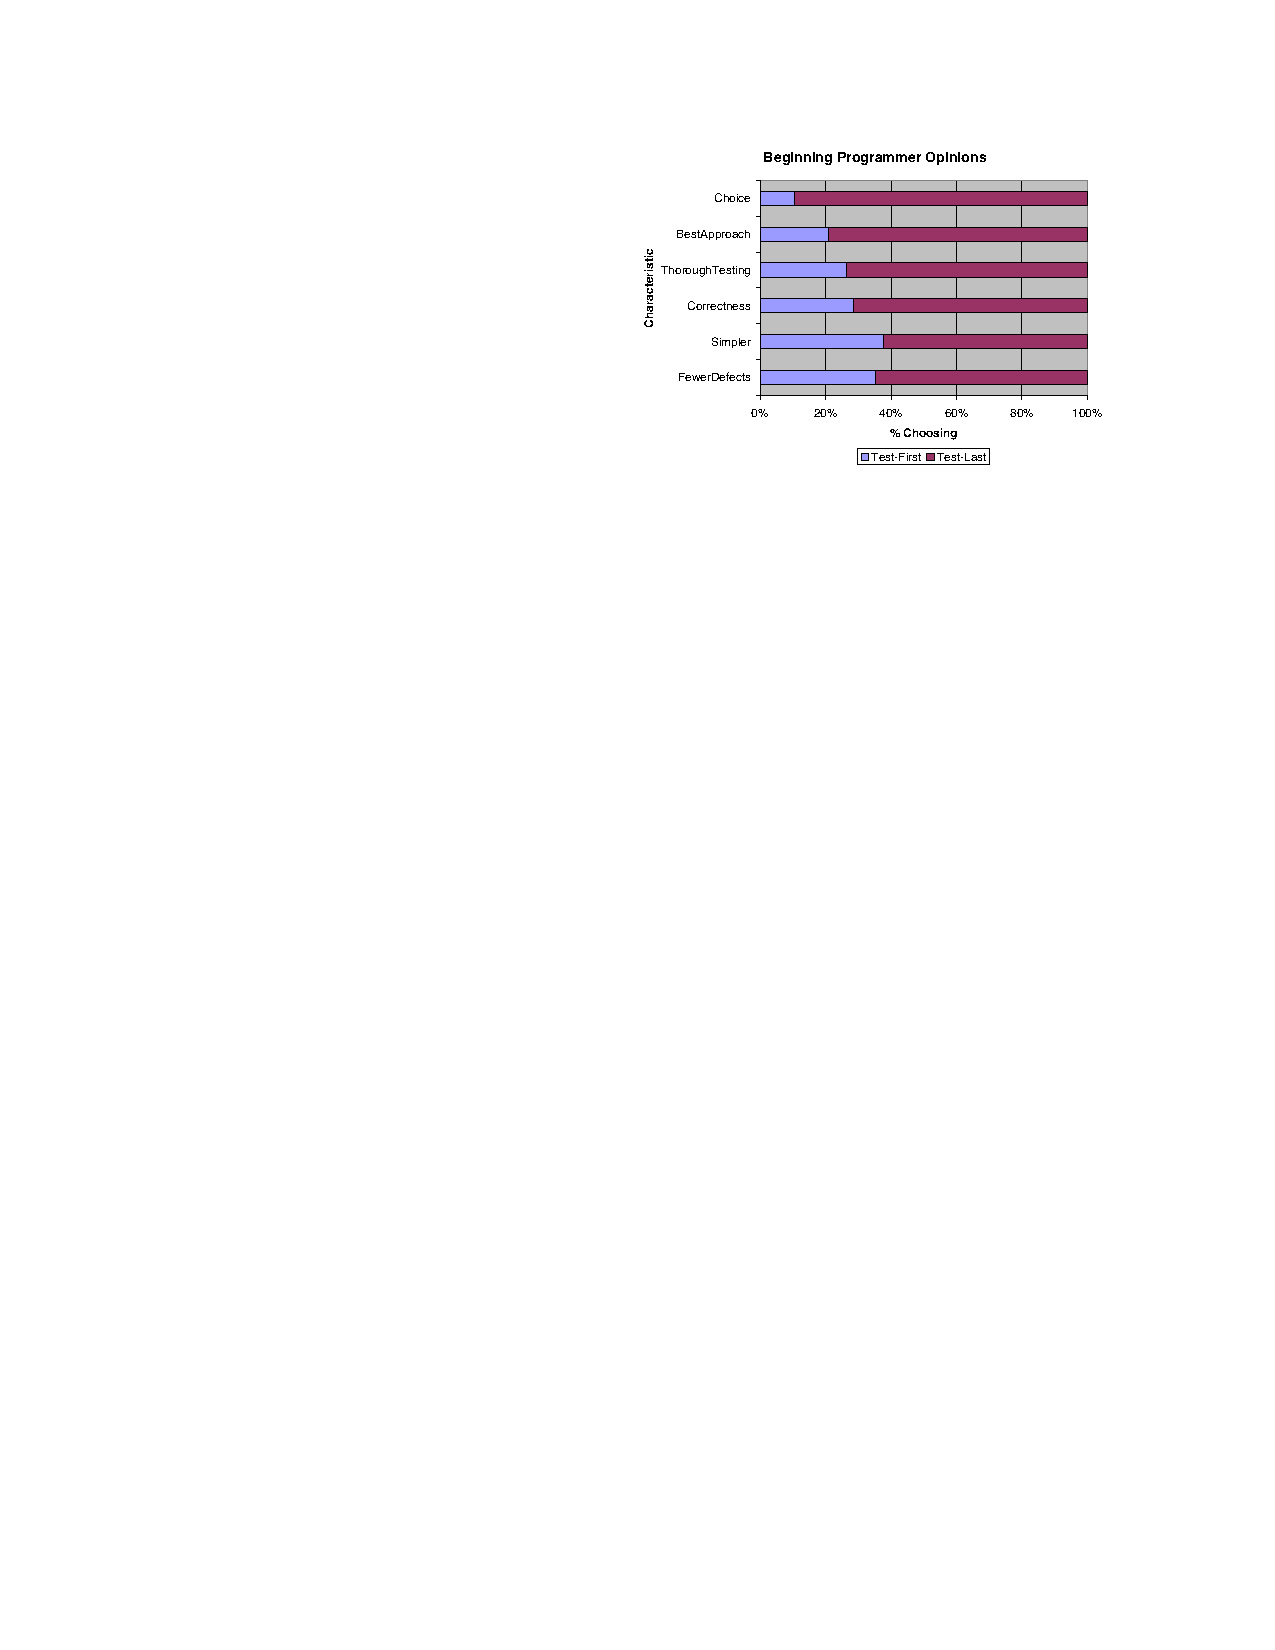
\psfig{file=janzengraph1.pdf,width =3in}
\caption{Results for beginner programmers in Janzen's study}
\end{figure}

\begin{figure}
\centering
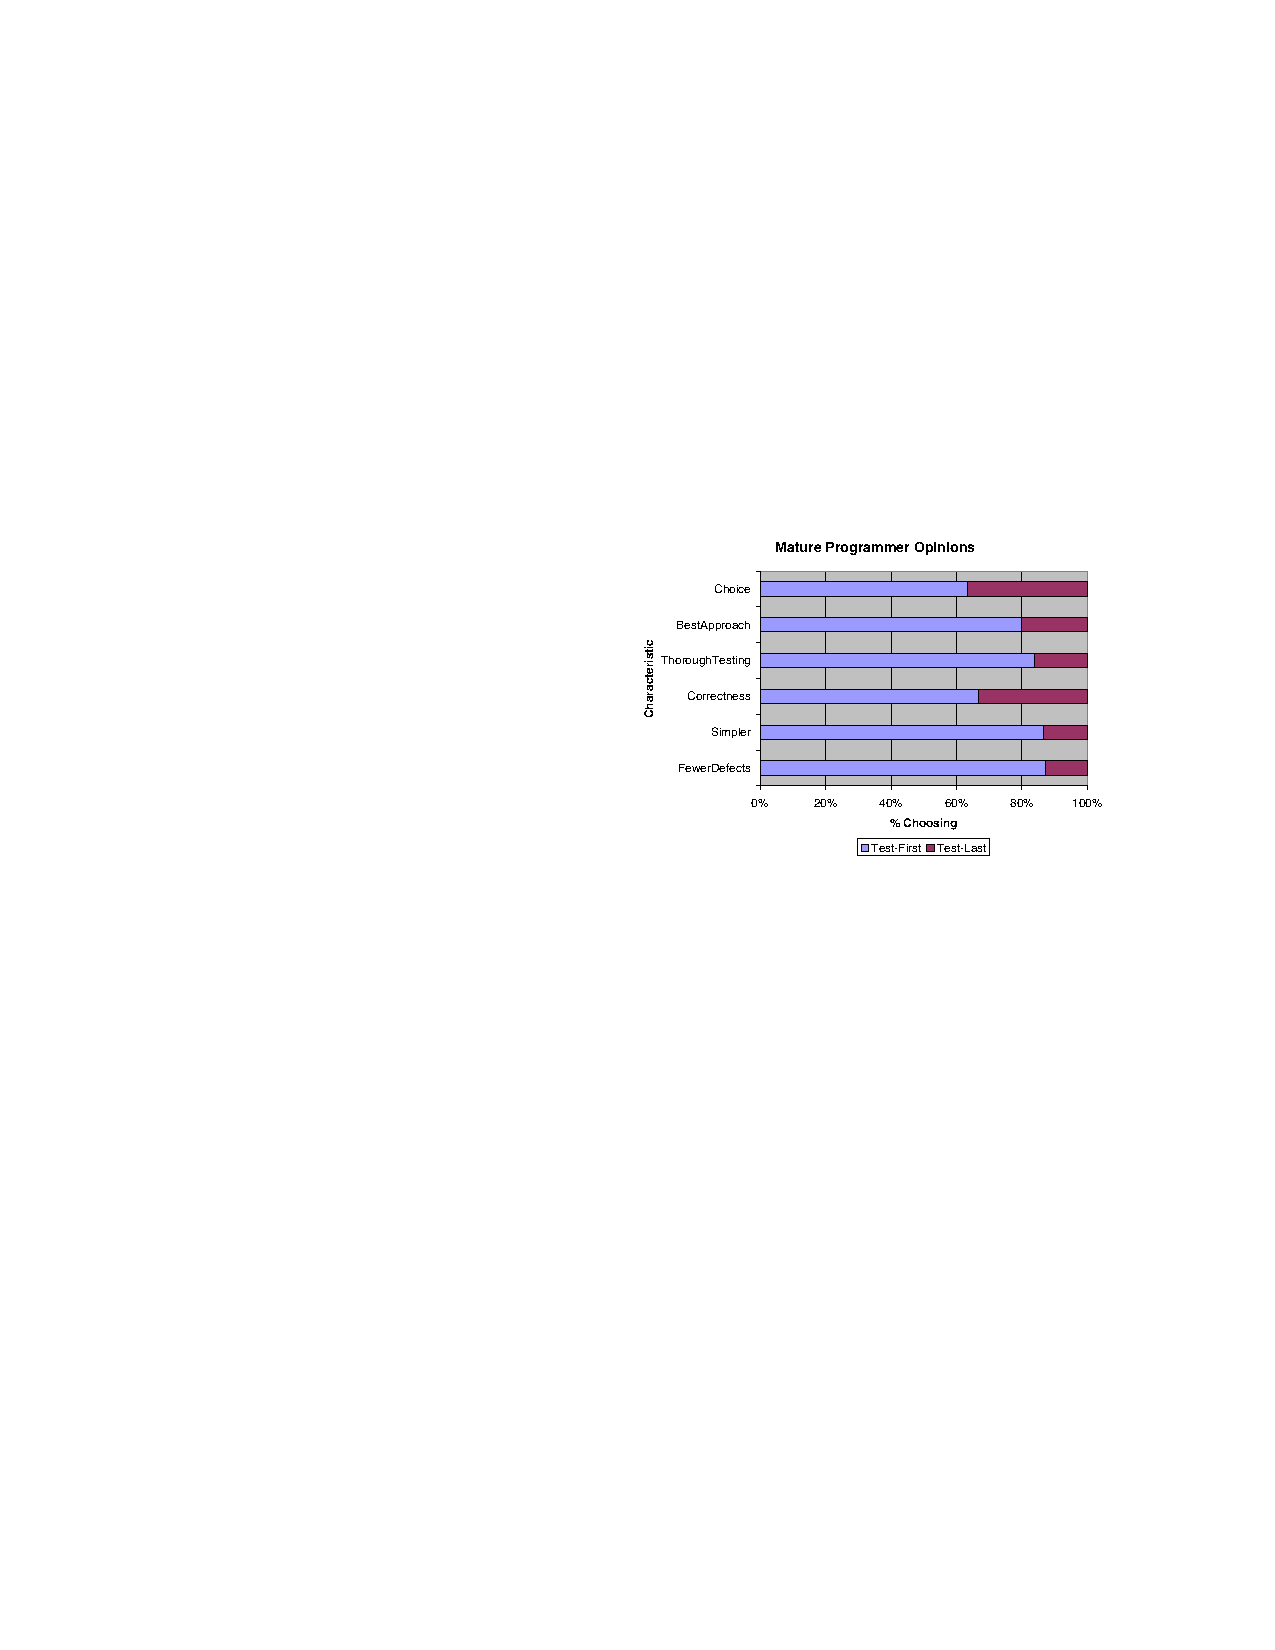
\psfig{file=janzengraph2.pdf,width =3in}
\caption{Results for Mature programmers in Janzens study}
\end{figure}

\subsubsection{Opinion Study by Janzen}

Last, is a 2007 opinion study by Janzen \cite{Janzen:2007}.  In this opinion study, Janzen polled participants from six experiments to determine whether they preferred testing with test-first methods or test-last methods.  Five of these experiments were conducted on students at the University of Kansas while one of the experiments was conducted on professional programmers from a Fortune 500 company.   Each participant was asked six questions where they had to choose between test-first and test-last testing.  The questions were:

\begin{itemize}
\item which approach they would choose in the future (\textbf{Choice})
\item which approach was the best for the project(s) they
completed (\textbf{BestApproach})
\item which approach would cause them to more thoroughly
test a program (\textbf{ThoroughTesting})
\item which approach produces a correct solution in less
time (\textbf{Correctness})
\item which approach produces code that is simpler, more
reusable, and more maintainable (\textbf{Simpler})
\item which approach produces code with fewer defects

(\textbf{FewerDefects})
\end{itemize}

The results were divided between a beginner group (students within their first few code classes) and a mature group (students nearing undergraduate graduation and professionals).  The results for the beginner group can be seen in figure 1 and the results for the mature group can be seen in figure 2.  Each graph shows the distribution of all of the participants answers to the six questions where each question is referenced by its bold keyword.  With the data given in the figures, Janzen was able to conclude that beginner coding students have a preference toward test-last testing while more mature coding students and industry professionals show no significant preference toward either testing method.  


%\subsection{Analysis}
%Two of the three studies covered the topic of code coverage.  In both studies by Kollanus and Lemos et al. it was acknowledged that increased test coverage had occurred in test-first testing methods compared to their test-last counterparts.  All three papers brought up total development time and noted that test-first testing tended to increase development time, although both Kollanus's review and Hellmann's review provide notable contradictory studies to this conclusion.   All three studies in one way or another also brought up code correctness in the form of external code quality in Kollanus or in the form of code quality in the case of Hellmann et al.  In this case the results were across the board where Lemos et al. stated that there was no code correctness difference between test first and test last whereas Kollanus said there was weak evidence that test-first testing, in the form of TDD, produces more correct code then test-last testing.  Hellmann et al provided contradictory evidence backing that in most studies test-first testing has shown better code correctness then test last testing but there was a noted study where test-first testing was less code correct then test-last testing.   In summary, with the studies given, test-first testing produces more code coverage and is likely to take more time to code then test-last testing but due to contradictions in the research given we can not draw a conclusion on code correctness.

\subsection{Understanding Contradictions}
Many summaries of TDD research ~\cite{Hammond:2012, Hellman:2012, Kettunen:2010, Kollanus:2010} have noted that studies that compare test-first to test-last testing tend to contradict one another.  Kollanus points out that articles in her review contradicted other articles which made it hard to make sound conclusions from the research given, especially on the subject of productivity.  The amount of contradictions concerned Kollanus enough that she noted the amount of contradictions as a potential confounding factor for her results.  Contradictions also existed between our review by Kollanus and our experiment by Lemos et al.  Although both articles seem to agree that code coverage is increased with test-first methods neither study seems to totally agree on the attributes of code correctness or total development time.  Since contradictions occur often in the results of our study we considered it to be important to explore some current theories on why these contradictions exist.  In particular we will be exploring two potential causes: method difficulty and improper study implementation/ documentation.

Method difficulty is considered a potential confounding factor when comparing test-first and test-last testing ~\cite{Hammond:2012, Kettunen:2010}. In particular, there is concern that test-first testing may be more difficult for beginning coders than test-last testing.  This is a concern because most study data comes from two sources with very different skill levels: industry professionals and college students.  In the study by Janzen et al, figures 1 and 2 show very different results between beginning and mature programmers.  In particular, beginner programmers did not report a very positive experience with test-first testing compared mature programmers.  This suggests that beginning coders may not be getting all the benefits from test-first methods that the more mature coders received.  If this is the case, then any summary method with mixed results between beginning and advanced programmers has a potential to have contradictory results.


The other problem that has plagued summary papers of test first testing is the lack documentation  and conformance of TDD methods in studies.  Kollanus, in her review paper, acknowledges a frustrating lack of information in many studies on how TDD was implemented.  Most articles, claimed Kollanus, had perhaps one or two lines describing their TDD methodology or only claimed that they used TDD.  Considering that TDD can be implemented in many ways, this lack of documentation for TDD implementation creates a problem in accurately comparing two studies.  This is an issue because multiple TDD methods may not preform equally, causing potentially contradicting results.  This problem could be avoided if studies documented their TDD process.  Another problem with TDD studies is that very few confirm their participants correctly implemented TDD~\cite{Hammond:2012}.  For example, in the study by Lemos et. al, the researchers acknowledged that one of their confounding factors was that they only asked students to write tests before code, thus a variety of different test-first methods might have been used within the study making its data less conclusive.   Overall the lack of documentation of how researchers specifically planned to implement TDD in their study and their lack of some sort of monitoring of whether the implementation was actually occurring greatly reduces the credibility of the experiment being done and allows for contradictory results to occur. 

\subsection{Conclusion}

Due to current issues in contradictory data it is hard to make solid conclusions about the advantages and disadvantages of using test-first testing instead of test-last testing.  That being said current trends exist within the research that allow us to guess some of the traits of test-first methods compared to test-last methods.  One result which was very clear in the research was that of code coverage.  The results from Lemos et al and Kollanus suggest that test-first testing tends to produce more code coverage compared to test-last testing. This seems to be a fairly uncontested conclusion as~\cite{Kettunen:2010, Hammond:2012} reached the same conclusion and no contradictions were found in other articles.  Another convincing trend that has occurred is that test-first testing seems to be harder to implement than test-last testing.  This trend is apparent from the results in Janzen and also from studies~\cite{Aniche:2010, George:2003} which will be discussed in the next section.     Although these trends seem to be clear, the rest seem to be more muddled.  Code correctness, for example, seems to have only a vague trend that agrees that test-first methods do not have worse code quality then test-last methods.  The debate about whether or not test-first testing produces better code correctness though has yet to be resolved due to conflicting data.  Another muddled trend is that of total development time.  Currently, the only thing that can be concluded on this topic is that test-first likely takes at least as much time as test-last methods to implement though it is unclear if test-first take significantly longer then test-last methods.

\section{Difficulty and TDD}
Due to TDD's popularity, almost all test first testing studies are done using TDD.  Because of this, the data for test-first testing has the potential to reflect an attribute of TDD that is not an attribute of test-first testing.  Although all the results found in the previous section have the potential to contain this issue, one particular result seems to suggest it may be a attribute of TDD and not test-first testing.  This attribute is the difficulty of test-first testing.  

\subsection{Studies noting TDD difficulty}
In 2012 Hammond et al did a summary paper on the current state of TDD.  In this paper Hammond et al states that: ``TDD remains deceptively simple to describe but deeply challenging to put into practice effectively"~\cite{Hammond:2012}.  Hammond et al defended their claim by summarizing several studies briefly that showed  the complexity of TDD.  In this section we will take a more in depth look at some of the studies Hammond et al used to draw their conclusion.  We will then in the next section discuss why these studies prove that the complexity is caused by the design of TDD and not test-first testing.

One of the studies that Hammond et al summarizes is the opinion study by Janzen.  In particular Hammond focuses on a quote from Janzens study: ``A few of the participants of the studies found TDD either too difficult or too different from what they normally do''.  This quote refers to an interesting relation found between the choice and best approach category.  It was noted by Janzen that in every experiment, there were more people who thought test-first was the best approach than people who would choose to implement test-first testing.  When Janzen looked into why this phenomena had occurred he found multiple statements in the comment section that claimed the difficulties of TDD and attributed the phenomena to TDD difficulty.

Another study that Hammond summarizes is a experiment survey by George and Williams~\cite{George:2003}.  In the study, multiple programming professionals from John Deere, RoleModel Software, and Ericsson participated in an experiment comparing TDD to waterfall development.  In this study a 9 question survey was given out asking programmers what they thought about TDD and what was difficult with TDD.  In this survey 56\% of the professionals noted that they had difficulty adapting to the TDD mindset when participating the study.  In addition 23\% of the participants noted that they felt that the lack of upfront design in TDD was more of a hindrance then a help. 

The last study Hammond summarizes in this portion of the paper is an online survey done by Aniche and Gerosa~\cite{Aniche:2010}.  In the survey, 218 TDD programmers of differing skill levels were surveyed about their TDD practices and mistakes.  In the survey, it was found that TDD was not easy to follow as about 25\% of the programmers admitted to frequently or always making mistakes in following the traditional steps of TDD.  Two examples of these mistakes include: forgetting to clean up their code after a test passes and writing tests that are too complex for effective TDD.
 
\subsection{Discussion}
The data above shows fairly strong evidence that TDD is at least somewhat difficult to implement but none of the data above shows that test-first testing is the problem.  In the first study, Janzen reveals that TDD was difficult for some people to implement.  In the second study, George and Williams reveal that 56\% of the participants found the TDD mindset hard to adapt while only 23\% of the participants found testing before designing as a problem, suggesting that something other then test-first testing caused difficulty for at least 33\% of the participants.  The third study showed that programmers had trouble implementing the steps of TDD, which has nothing to do with testing before designing.  With these studies in mind, difficulty in using TDD does not seem to be directly linked with test-first testing.  This suggests that a different issue is causing TDD to be difficult to implement.

One potential issue with TDD that is brought up by many developers is that it fails to explain how to write good test-first tests.  This is best represented in a quote from Dan North's article~\cite{North:xxx}: ``While using and teaching agile practices like test-driven development (TDD) on projects in different environments, I kept coming across the same confusions and misunderstandings. Programmers wanted to know where to start, what to test and what not to test, how much to test in one go, what to call their tests, and how to understand why a test fails."  In this quote Dan North expresses his and other coders frustration with TDD and its failure to specify how and what tests should be written.  This problem is also mentioned in articles~\cite{Kettunen:2010, Seoken:2012}.  Currently their is no empirical evidence that this could be the cause of the TDD difficulty, but it is currently suspect by knowledgeable experts in the field. 

\section{Evolutions of TDD}

New test-first methods are starting to appear in the agile community that contain some of TDD's main tenets but are different enough from TDD that they are starting to receive their own names and classifications.  These new methods are starting to appear because many developers in one or another are not satisfied with the current implementation of TDD.  In this subsection we will discuss one of these popular TDD spin-offs, behavior driven development, which was developed to combat the problem noted in the previous paragraph.

%\subsection{Acceptance Test Driven Development}

%Perhaps the closest spin off to TDD, acceptance test driven development (ATDD), follows many of the ideas and expectations that regular TDD does, like writing tests first and using tests to define the development code.  Unlike TDD, though, ATDD believes that in order to produce higher quality code and reduce code, customers should write or define "acceptance" tests.  These acceptance tests are tests that are required to pass before the customer will accept the product and usually define the core functionality of the product being developed.  This part of ATDD is noticeably different from the TDD ideology because in the TDD ideology only the developer should writes the tests and the tests should be written from simplest to hardest.~\cite{Hammond:2012}

%The shift from having the developer write all the tests to the customer having to write some of tests is ideally considered a win win.  The shift of the workload of determining main functionality from the developer to the customer significantly reduces the difficulty of the TDD practice to the developer as they are no longer concerned about writing and determining all the functionality for their code.  This method is also supposed to benefit the customer as it allows the customer to get the product they desire.  One of the major complaints of ATDD is that it is an ideal practice at best because customers will not take the time to create useful acceptance tests.~\cite{Hammond:2012} Another complaint of ATDD is that its very hard for  customers to write useful acceptance tests  because they view functionality differently then developers because their knowledge of code is limited.(site new IEEE article here)  Because of these varied complaints, some of the promoters of ATDD have moved away from it to support a newer similar TDD spin off, Behavior Driven Development.

Behavior Driven Development, or BDD for short, was created by Dan North as a substitution for TDD that helps the user determine what to test and how to test it.  The main difference between BDD and TDD is that TDD focuses on testing the code itself while BDD focuses more on testing a codes intended behavior. In order to do this, BDD users start by considering their codes intended functionality.  They then sentences that use their native language to define what they want their code to achieve.  These sentences are then converted from the programmers native language to tests in a standard testing language using various programming tools and methods that have been developed specifically for BDD \cite{Soeken:2012, North:xxx, Hammond:2012}. This differs from TDD because the focus is no longer on testing new features but on defining what these new features should do.  This shift in focus and use of native language to define problems, according the Dan North, is what makes BDD simpler to implement. \cite{North:xxx}

\section{conclusion}
\subsection{Summary}

In this paper we talked about and compared two common test methods: test-first testing and test-last testing.  Within this discussion we reviewed current research in the field in an attempt to make conclusions about the advantages and disadvantages of test-first and test-last methods.  In this part of the paper we were somewhat able to conclude that test-first testing increases code coverage, is more difficult to implement, has at least as much code correctness, and takes at least as long to develop as test-last testing.  These conclusions must be considered weak though as we noted that studies were very contradictory to one another due to various factors including method difficulty and poor study design/documentation.  We also discussed how there seems to be evidence that being harder to implement is not a problem with test-first testing but with TDD, the way test first testing is usually implemented.  We ended by exploring a new test-first method that had the potential to fix this issue with TDD.

\subsection{Suggested Further Research}
For people who are looking to increase clarity in the debate between test-first and test-last testing there are a few studies that would be quite useful in its current state.  One helpful study that could be implemented is a summary study of TDD and test-first testing articles which are divided up by participant coding expertise to see if participants with different programing experience achieve differing results.  Another useful study that could be implemented would be to compare the new BDD method against TDD to see if participants find BDD simpler to implement than TDD.  Also any new research on the debate that has a well documented TDD method and has some way to confirm that participants preformed this method would be useful in helping to solve the debate by giving it more creditable studies to work with.


\bibliographystyle{abbrv}
% sample_paper.bib is the name of the BibTex file containing the
% bibliography entries. Note that you *don't* include the .bib ending here.
\bibliography{Paper_Draft}  
% You must have a proper ".bib" file
%  and remember to run:
% latex bibtex latex latex
% to resolve all references

\end{document}
